\section{Benutzerhandbuch}
\subsection{Einleitung}

Das Digital Input Computer Keyboard ist eine Art elektronisches Keyboard, dass verschiedene Samples abspielen und aufnehmen kann. Man kann mithilfe der gegebenen Samples (Piano und Schlagzeug) spielen und Tonspuren aufnehmen. Aufgenommene Tonspuren können dann auch parallel abgespielt werden. Es können aber auch eigene Samples in das Programm geladen werden. Mit diesen kann man ebenso verfahren wie mit den gegebenen.

\begin{figure}[hbtp]
\centering
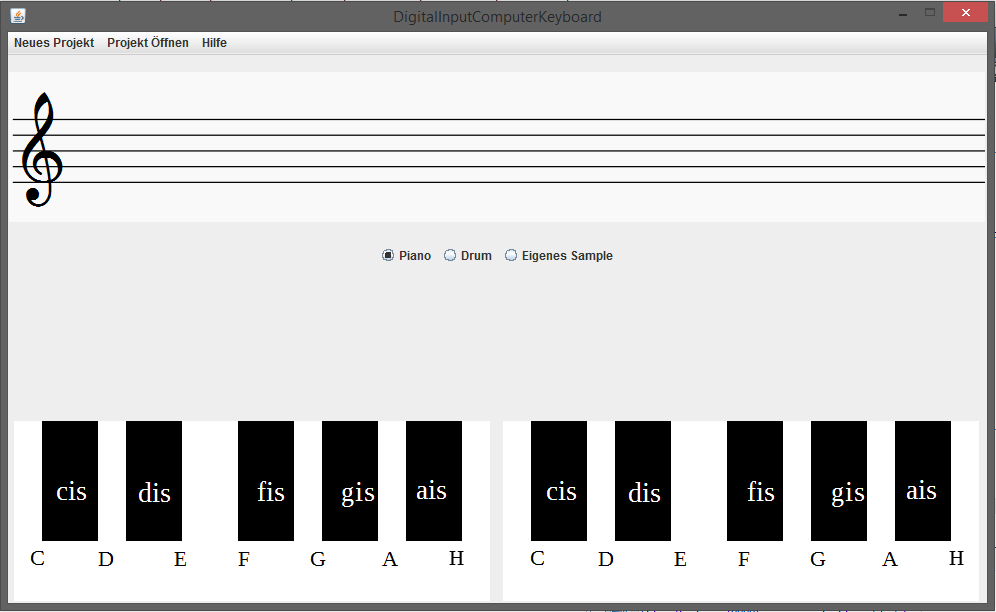
\includegraphics[scale=0.6]{Bilder/Projektbild1.PNG} 
\caption{Bild der Benutzeroberfläche}
\end{figure}


\subsection{Projekt}

Mithilfe des DICKs hat man die Möglichkeit Projekte zu erstellen. Ein Projekt enthält dann ein Projektfile, einen Ordner in dem eigene Aufnahmen abgespeichert sind und einen Sample Ordner in den man eigene Samples hinein laden kann.

\newpage


\subsubsection{Erstellen}

Mithilfe des Buttons "Neues Projekt" kann man einen Projekt Ordner erstellen. Dieser Ordner muss erst benannt und dann ein Speicherort ausgewählt werden. Während der Namensgebung aktivieren sich die Tasten, dies kann aber ignoriert werden. 

\begin{figure}
	\subfigure[Neues Projekt -Button]{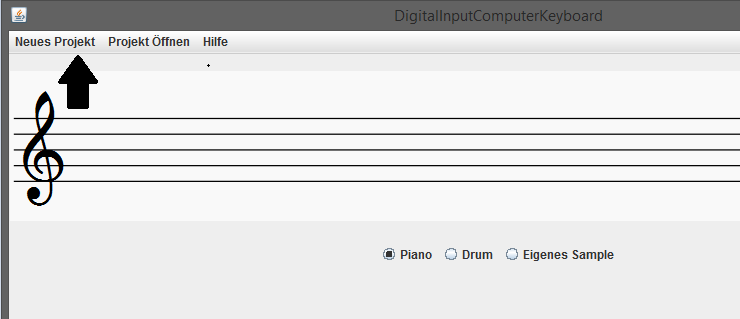
\includegraphics[width=0.49\textwidth]{Bilder/Projektbild2_1.PNG}}
	\subfigure[Eingabe-Feld für den Projektname]{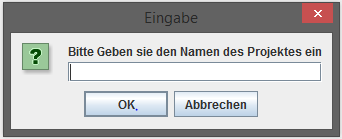
\includegraphics[width=0.49\textwidth]{Bilder/ProjektEingabeName.PNG} }
\caption{Projekt Erstellen}
\end{figure}

Sobald das Projekt benannt wurde muss nur noch ein Speicherort ausgewählt werden.

\begin{figure}[hbtp]
\centering
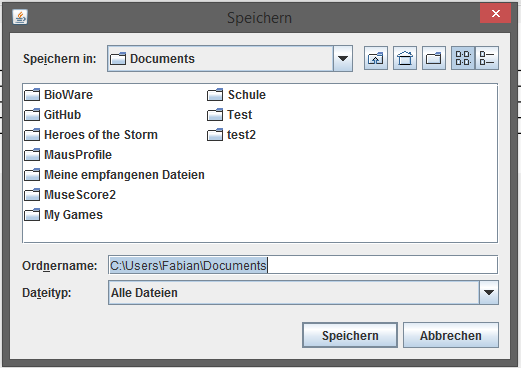
\includegraphics[scale=1]{Bilder/ProjektSpeichern.PNG}
\caption{Speicherplatzauswahl}
\end{figure}



\subsubsection{Öffnen}

Wenn man bereits ein Projekt erstellt hat kann man dieses mithilfe des Buttons "Projekt Öffnen" öffnen. Man sucht den Projekt Ordner und wählt die Projektfile.bin aus. Sobald dies erledigt wurde, öffnet sich ein separates Fenster in dem man weitere Funktionen zur Auswahl hat.

\begin{figure}[hbtp]
\centering
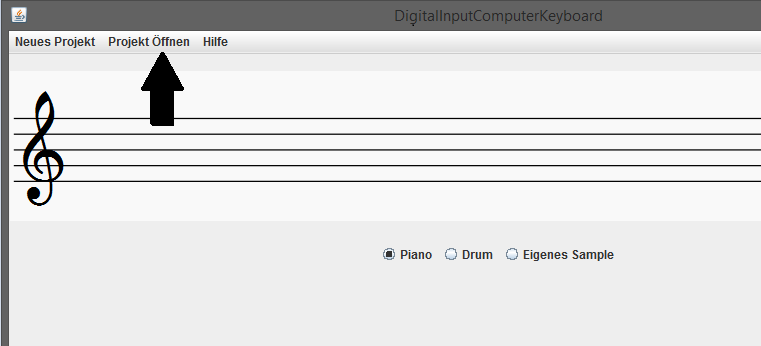
\includegraphics[scale=0.6]{Bilder/Projektbild3_1.PNG}
\caption{Der Button Projekt Öffnen}
\end{figure}

\newpage




\subsubsection{Aufnehmen}

Sobald man ein Projekt erstellt und geöffnet hat, kann man gespieltes Aufnehmen. Dazu muss man das Tempo und den Namen der Datei eingeben die aufgenommen werden soll. Zu beachten ist hierbei dass man sobald der Name oder das Tempo eingegeben wurde Enter gedrückt wird, da diese während dem spielen sonst verändert werden.

\begin{figure} 
    \subfigure[Eingabe-Feld für den Dateiname]{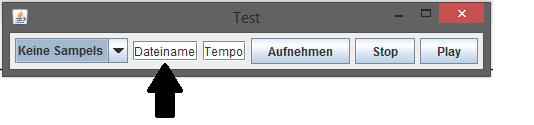
\includegraphics[width=0.49\textwidth]{Bilder/Projektbild4_Dateiname.PNG} } 
    \subfigure[Eingabe-Feld für das Tempo]{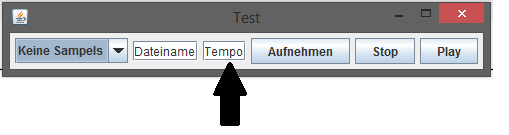
\includegraphics[width=0.49\textwidth]{Bilder/Projektbild4_Tempo.PNG} } 
    \subfigure[Aufnehmenbutton]{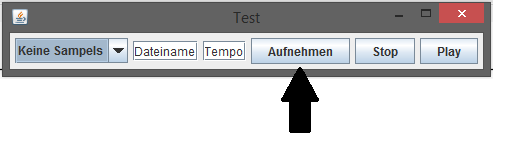
\includegraphics[width=0.49\textwidth]{Bilder/Projektbild4_AufnehmenButton.PNG} } 
\caption{Aufnahmespezifische Bedienelemente} 
\end{figure}

Sobald alles ausgefüllt wurde muss man den Aufnehmenbutton betätigen. Es folgen vier einleitende Schläge in dem gewählten Tempo bevor aufgenommen wird. Um die Aufnahme wieder zu stoppen einfach den Stopbutton betätigen.

\begin{figure}[hbtp]
\centering
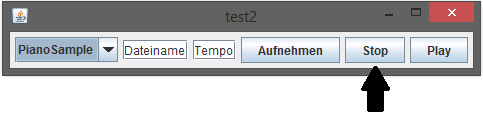
\includegraphics[scale=1]{Bilder/Projektbild4_Stop.PNG}
\caption{Der Stopbutton}
\end{figure}

\newpage


\subsubsection{Abspielen}

Um ein aufgenommenes Sample abzuspielen betätigt man den PlayButton. Dadurch öffnet sich ein Fenster in dem man seine aufgenommenen Samples sieht.

\begin{figure}[hbtp]
\centering
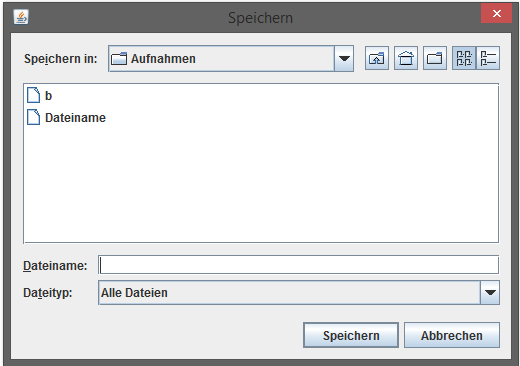
\includegraphics[scale=0.8]{Bilder/AbspielenBild.PNG}
\caption{Das Fenster in dem gespeicherte Samples angezeigt werden}
\end{figure}


Durch Auswahl einer Aufnahme wird ein Fenster geöffnet das einen Button enthält. Durch betätigen des Buttons wird das Sample abgespielt. Dabei werden die aufgenommenen Noten angezeigt. Hier wurde beispielhaft die Aufnahme b geöffnet.

\begin{figure}[hbtp]
\centering
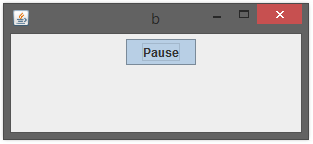
\includegraphics[scale=0.9]{Bilder/abspielenbsp.PNG}
\caption{Das Abspielen Fenster eines Samples}
\end{figure}

Um die Aufnahme nun abzuspielen muss man nur noch den Pausebutton betätigen. Durch nochmaliges betätigen wird das abspielen angehalten und kann durch erneutes betätigen fortgesetzt werden.\\

\textbf{Anmerkung:} Wenn mehrere Aufnahmen geöffnet sind und gleichzeitig abgespielt werden wollen, kann man dies mithilfe der Leertaste tun.


\subsubsection{Eigene Samples}
 
 
 Um eigene Samples in das Programm einzufügen muss man diese in den Sample Ordner des Projekt einfügen. Dabei muss man einige Dinge beachten:
 
 \begin{itemize}
   \item[•] Die Töne des Samples müssen 8 oder 16 bit lang sein.
   \item[•] Es müssen wav Dateien sein.
   \item[•] Alle Töne eines Samples müssen in einem eigenem Ordner abgelegt sein
   \item[•] Die Töne müssen wie folgt bezeichnet sein:
   			\begin{itemize}
   			
   				\item[-] A4
   				\item[-] A5
   				\item[-] Ais4
   				\item[-] Ais5
   				\item[-] B4
   				\item[-] B5
   				\item[-] C4
   				\item[-] C5
   				\item[-] Cis4 
   				\item[-] Cis5
   				\item[-] D4
   				\item[-] D5
   				\item[-] Dis4
   				\item[-] Dis5
   				\item[-] E4
   				\item[-] E5
   				\item[-] F4
   				\item[-] F5
   				\item[-] Fis4
   				\item[-] Fis5
   				\item[-] G4
   				\item[-] G5
   				\item[-] Gis4
   				\item[-] Gis5
   				   				
   			\end{itemize}
   	
   
 \end{itemize}            
             
\newpage

     Wenn diese Bedingungen erfüllt sind sollte das Sample in dem Dropdownmenü auswählbar sein.
     
     \begin{figure}[hbtp]
     \centering
     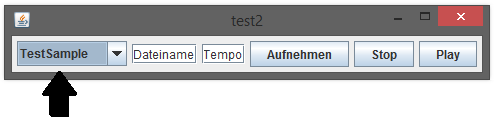
\includegraphics[scale=1]{Bilder/SampleDropdown.PNG}
     \caption{Dropdownmenü}
     \end{figure}
     
             
             
\textbf{Anmerkung:}\\

Ein Sample im Dropdownmenü auszuwählen reicht noch nicht aus. Zusätzlich muss in der Benutzeroberfläche Eigene Samples ausgewählt sein, da sonst das entsprechende schon in dem Programm integrierte Sample abgespielt wird.

\begin{figure}[hbtp]
\centering
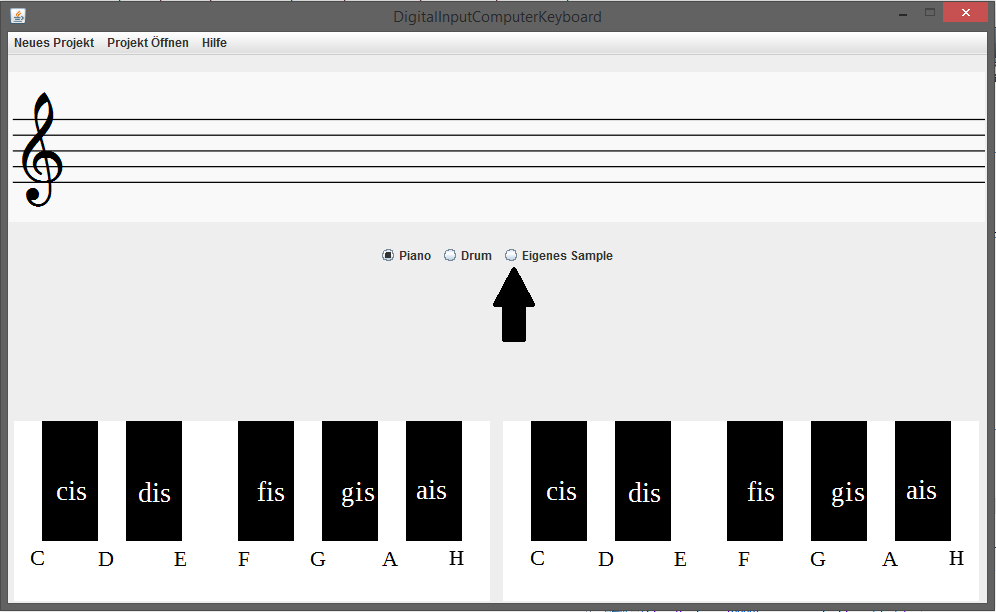
\includegraphics[scale=0.6]{Bilder/Projektbild1EigenesSample.PNG}
\caption{Eigenes Sample auswählen}
\end{figure}

             
             
             
             
             
             
             
             
             
             